\scanpage{51}
L'image inverse de $\xi$ dans $H^1(S,N_1)$ est en correspondance biunivoque avec l'ens des Tores maximaux de $G$, modulo automorphismes intérieurs. En particulier, il est non vide \deleted{\unsure{ssi}} i.e. on peut restreindre le groupe structural à $N_1$, ssi il existe un tore maximal; s'il en est ainsi, alors il est réduit à un élément ssi tous les tores maximaux sont conjugués, [ce qui n'est vrai que exceptionnellement dans des situations ``arithmétiques''].

\margin{Vaut \deleted{\unsure{pour}} \unsure{sans supposer} \unsure{seulement} que $G_1$ \unsure{ait un tore maximal}.}
\margin{\figure{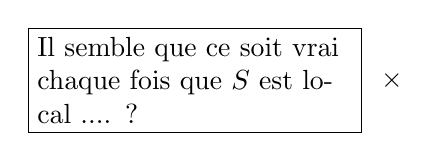
\begin{tikzpicture}\node[draw,align=left,text width=4cm] {Il semble que ce soit vrai chaque fois que $S$ est local .... ?};\node at (2.5,0) {$\times$};\end{tikzpicture}}}

\margin{\deleted{\unsure{donc}} Si $S$ local, \deleted{$T_1\ \unsure{est déployé}$}, $N_1$ produit \unsure{semi-direct} de $W_1=W_0$ \unsure{et} $T_1$, on a
\diagram{\begin{tikzcd}[ampersand replacement=\&]H^1(S,N_1)\arrow[r,"\text{surj}"]\&H^1(S,W_0)\end{tikzcd}}.
\unsure{Le résultat} \deleted{\unsure{précédent}} \unsure{se démontre} \deleted{\unsure{ainsi}} si on est \unsure{sur un} \unsure{anneau} \unsure{de} \deleted{\unsure{Tores}} \unsure{locaux}; exprimer qu'un élément de $H^1(S,W_0)$ donne \unsure{l'image} $\xi$ \deleted{\unsure{neutre}}.}
\margin{\figure{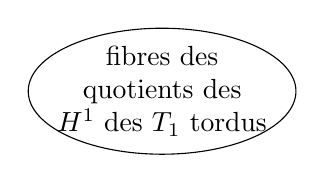
\begin{tikzpicture}\node[align=center] at (0,0) {fibres des\\quotients des\\$H^1$ des $T_1$ tordus};\draw (0,0) ellipse (1.7 and .8);\end{tikzpicture}}}

L'image inverse de $\xi$ dans $H^1(S,\unsure{\overline N_1})$ est en correspondance biunivoque avec l'ens des couples $(T\subset B)$ de Killing dans $G$, modulo aut. extérieurs; Donc il est non vide ssi il existe un tel couple, ou encore s'il existe un Tore \deleted{privilégié} de Chevalley, ou encore un Borel de Chevalley, \inserted{[donc exceptionnel \unsure{dans des cas arithmétiques}];} et \deleted{\unsure{dans ce cas}} s'il en est ainsi, alors l'ens est réduit à un élément ssi \deleted{\unsure{deux}} couples de Killing de $G$ sont conjugués.
[et il est probable que cette condition soit vérifiée sur tt anneau local; c'est évidemment le cas si on suppose de plus $T_1$ trivial \inserted{[i.e. $\rho=0$]}, par le lemme de \unsure{Bru---}]

\margin{Question équivalente : les \unsure{ss-groupes} \unsure{de} \deleted{\unsure{paraboliques}} Borel sont conjugués ? \unsure{Dans un Tore} \unsure{maximal} d'un \uline{Borel $B$} \unsure{sont ils toujours} conjugués \unsure{dans $G$} \uline{dans $B$}}
\margin{50}
